%\documentclass[12pt,a4paper,twoside,draft]{report}
\documentclass[12pt, a4paper]{report}
\usepackage[T2A]{fontenc}
\usepackage[utf8]{inputenc}

\usepackage[main=russian,english]{babel}
\usepackage{amssymb}
\usepackage{amsmath}
\usepackage{amsthm}
\usepackage{epsfig}
\usepackage{array}
\usepackage{longtable}
\usepackage{tabularx}
\usepackage{subfigure}
\usepackage{fancyheadings}
\usepackage{ccfonts}
\usepackage{psfrag}
\usepackage{cite}
\usepackage{euscript}
\usepackage{graphicx}
\usepackage{wrapfig}
\usepackage{epstopdf}
\usepackage[rflt]{floatflt}
\usepackage{floatrow}

\sloppy
\pagestyle{plain}

\newcounter{TaskNumber}
\setcounter{TaskNumber}{1}

\renewcommand{\thesection}{\arabic{section}.}
\renewcommand{\thesubsection}{\arabic{section}.\arabic{subsection}}

% Определяем недостоющие операторы
\DeclareMathOperator*{\argmin}{argmin}
\DeclareMathOperator*{\Argmin}{Argmin}

\theoremstyle{definition}
\newtheorem*{Definition}{Определение}
\theoremstyle{plain}
\newtheorem*{Theorem}{Теорема}
\newtheorem*{Lemma}{Лемма}
\theoremstyle{remark}
\newtheorem*{Remark}{Замечание}
\newtheorem*{Example}{Пример}
\newtheorem*{Consequence}{Следствие}
\theoremstyle{remark}
\newtheorem*{Task}{Задание}
\theoremstyle{definition}
\newtheorem*{ProblemStatement}{Постановка задачи}

\addto\captionsenglish{ \renewcommand*\contentsname{Содержание}}
\addto\captionsenglish{\renewcommand{\figurename}{Рис.}}
\addto\captionsrussian{\def\refname{Список используемой литературы}}


\author{Zavgorodniy Igor, 442}
\title{Отчёт}
\date{}

%\includeonly{Title,0-Introduction,Ch1,Ch2,Ch3,Conclusion,Bibliography}


\begin{document}
\begin{titlepage}
  \begin{center}
    \large
    МОСКОВСКИЙ ГОСУДАРСТВЕННЫЙ УНИВЕРСИТЕТ\\ имени М.В.ЛОМОНОСОВА\\
    ФИЗИЧЕСКИЙ ФАКУЛЬТЕТ\\КАФЕДРА ФИЗИКО-МАТЕМАТИЧЕСКИХ МЕТОДОВ УПРАВЛЕНИЯ

	\underline{\hspace{12cm}}

    \vfill

    {\LARGE \textbf{Специальный физический практикум:
 \\ управление динамическими объектами}}
  	\bigskip
  	
    {\textbf{Система управления положением антенны}}  	
  	\bigskip


    Отчёт студента IV курса\\
    Завгороднего Игоря Викторовича
\end{center}
\vfill

\begin{flushright}
Преподаватель:\\
Митришкин Ю.В.
%$\labda$
\end{flushright}
\vfill

\begin{center}
  Москва\\2018
\end{center}
\end{titlepage}

\newpage
\tableofcontents

%Постановка задачи управления
%Описание линейной модели объекта
%Анализ системы
%Синтез PID-регулятора
%Дополнительно исследование системы
%Вывод
%Приложение
%Список литературы

\newpage
\section{Постановка задачи управления}
Передо мной стояла задача синтезировать такой регулятор для системы, для которого при заданном входном сигнале, $r(t)=Bt$, установившаяся ошибка не превышала бы $0,01B$. А в случае ступенчатого входного сигнала перерегулирование не превышало $5\%$, а время установления (по критерию $2\%$ ) должно быть менее 2 с. \\
Кроме того, требовалось построить график переходной харатеристики системы и, полагая $R(s)=0$, определить влияние возмущения $D(s)=Q/s$  на выходную переменную $Y(s)$.\\
Синтез регулятора осуществлялся в среде SIMULINK, входящей в комплекс Matlab.\\
Мне удалось найти необходимые параметры, а также исследовать поведение системы при различных входных данных.\\
Давайте рассмотрим ход работы и проанализируем полученные результаты.


\section{Описание линейной модели объекта}
\label{sec:W1}

Большая антенна предназначена для приёма сигналов со спутника. Она должна с высокой точностью следить за изменением его положения на орбите. Система управления антенной включает в себя двигатель, увправляемый по цепи якоря, и регулятор, который требуется синтезировать.

\section{Анализ системы}
Прежде чем мы приступим к выполнению задачи, нам следует получить некие сведения о системе. \\
Рассмотрим, как работает разомкнутая система без регулятора. После
использования команды step реакция системы на “ступеньку” растет неограниченно, а команда  isstable возвращает 0,  что говорит о неустойчивости системы. 

 \begin{figure}[h!]
    \center{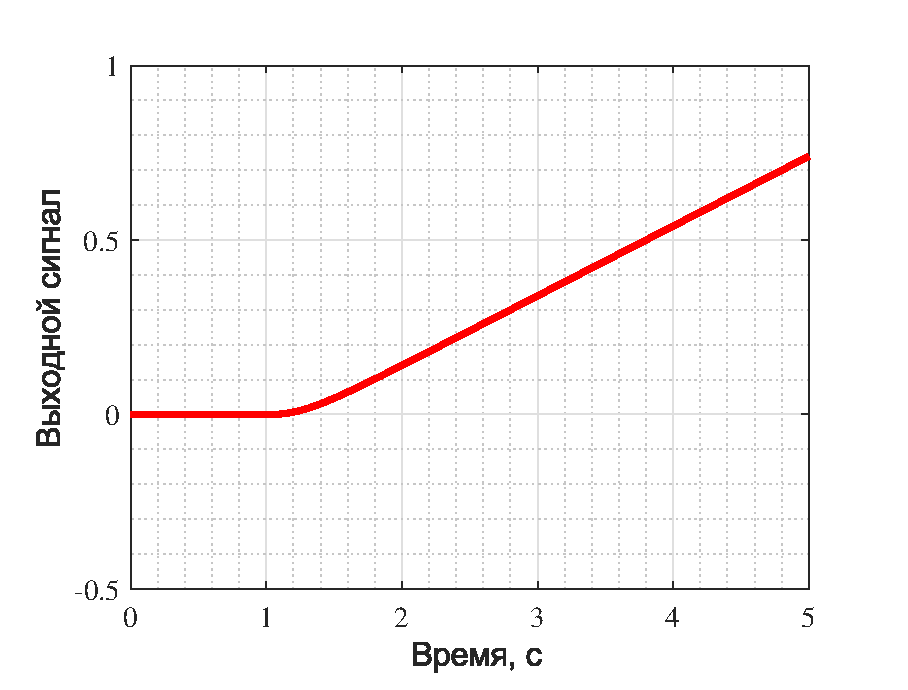
\includegraphics[scale = 0.85]{OpenSysStepReact.eps}}
    \caption{Реакция разомкнутой системы на ступеньку}
\end{figure}

\newpage
Очевидно, что это противоречит нашим требованиям, сформулированным в
постановке задачи.\\
Рассмотрим теперь замкнутую систему, которая выглядит следующим
образом:

 \begin{figure}[h!]
    \center{\includegraphics[scale = 0.85]{scheme.png}}
    \caption{Система управления положением антенны}
\end{figure}

Для определённости возьмём $Q=0.0001$ и $Reg=1$. Реакция данной системы на единичную ступеньку 
выглядит следующим образом: 

 \begin{figure}[h!]
    \center{\includegraphics[scale = 0.85]{CloseSysStepReact.eps}}
    \caption{Реакция замкнутой системы на ступеньку}
\end{figure}

\newpage
Далее найдем все полюса системы. Как видно из рисунка 4 у системы все полюса системы вещественные. 
Нулевой полюс находится на границе устойчивости, влияние остальных на поведение системы заметно ниже.

 \begin{figure}[h!]
    \center{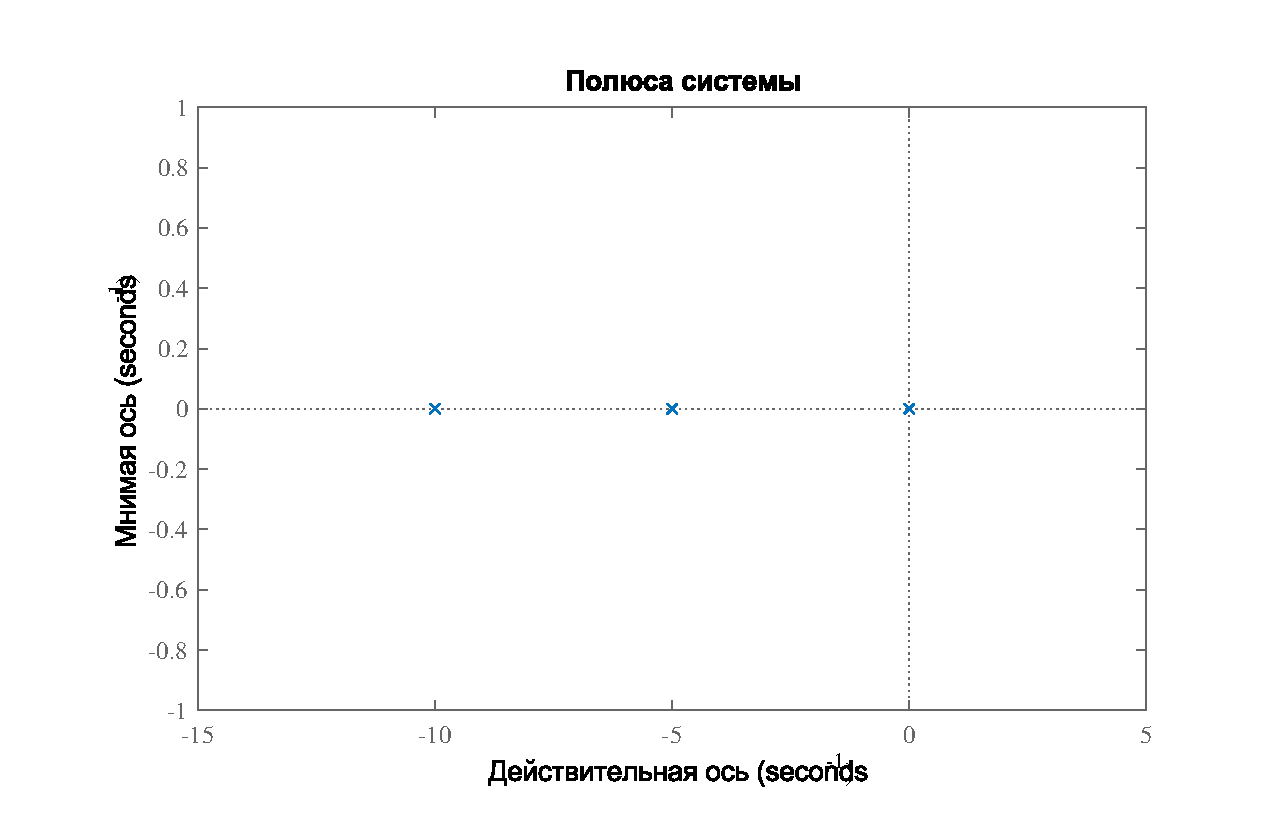
\includegraphics[scale = 0.6]{ploes.eps}}
    \caption{Полюса передаточной функции}
\end{figure}

\section{Синтез PID-регулятора}
Пропорционально-интегрально-дифференцирующий (ПИД) регулятор —
устройство в управляющем контуре с обратной связью. Используется в
системах автоматического управления для формирования управляющего
сигнала с целью получения необходимых точности и качества переходного
процесса. ПИД-регулятор формирует управляющий сигнал, являющийся
суммой трёх слагаемых, первое из которых пропорционально разности
входного сигнала и сигнала обратной связи (сигнал рассогласования), второе
— интеграл сигнала рассогласования, третье — производная сигнала
рассогласования.\\
Напомним, что на вход системе подаётся линейно возрастающий сигнал $r(t)=Bt$, для удобства возьмём коэффицент 
$B=13$, таким образом мы должны добиться соблюдения следующих условий:\\
\begin{itemize}
  \item установившаяся ошибка не должна превышать $0,13$;
  \item в случае ступенчатого входного сигнала перерегулирование не должно превышать $5\%$;
  \item  время установления (по критерию $2\%$ ) должно быть менее 2 с.
\end{itemize}

Передаточная функция ПИД-регулятора в общем случае выглядит так:
 \begin{align}
  Reg(s)=K_{P}+K_{I}\frac{1}{s}+K_{D}\frac{N}{1+N\frac{1}{s}}
\end{align}
1при помощи функций pidtool и
pidtune в среде Matlab, были получены следующие значения для
коэффициентов:
\begin{itemize}
  \item $K_{P}=17.4851130836651$;
  \item $K_{I}=0.916494149876436$;
  \item $K_{D}=8.87298672654388$;
  \item $N=703.826906485883$;
  
 \end{itemize}
 
 Установившаяся ошибка стремится к нулю со временем:
 \begin{figure}[h!]
    \center{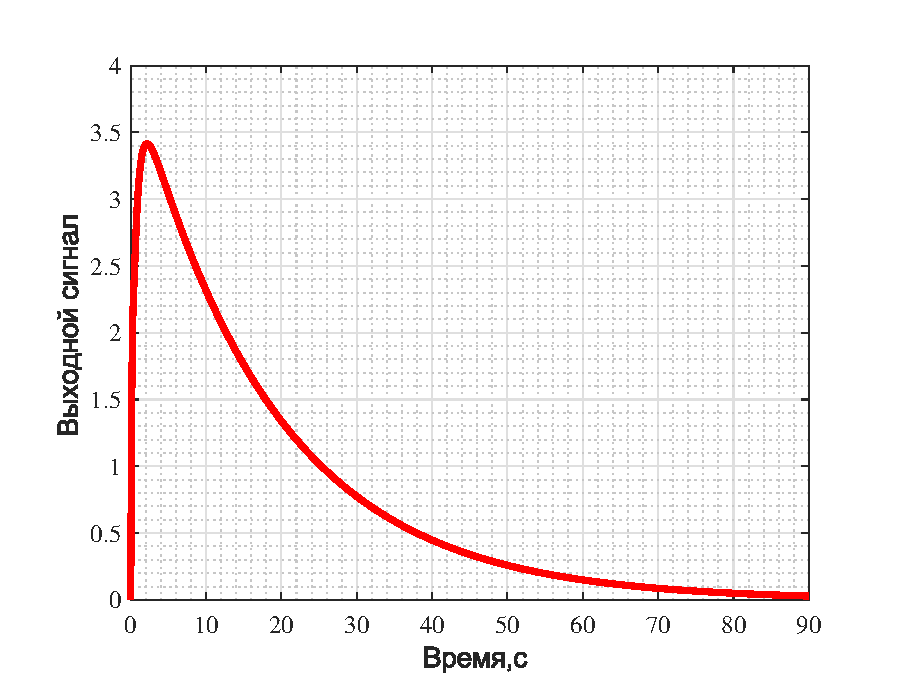
\includegraphics[scale = 0.85]{LinError.eps}}
    \caption{Установившаяся ошибка}
\end{figure}

После построения системы управления были измерены следующие
показатели:
\begin{itemize}
  \item Время нарастания (rise time)=0,687 сек.;
  \item Время установления (settling time)=1,55 сек.;
  \item Коэффициент проскакивания (overshoot) = 0,97\%;
  \item Запас по амплитуде (gain margin) = 40,4 dB @ 95,9 rad/s;
  \item Запас по фазе (phase margin) = 79,2 deg @ 6,16 rad/s;   
  \item Система устойчива.
 \end{itemize}
 
 \begin{figure}[h!]
    \center{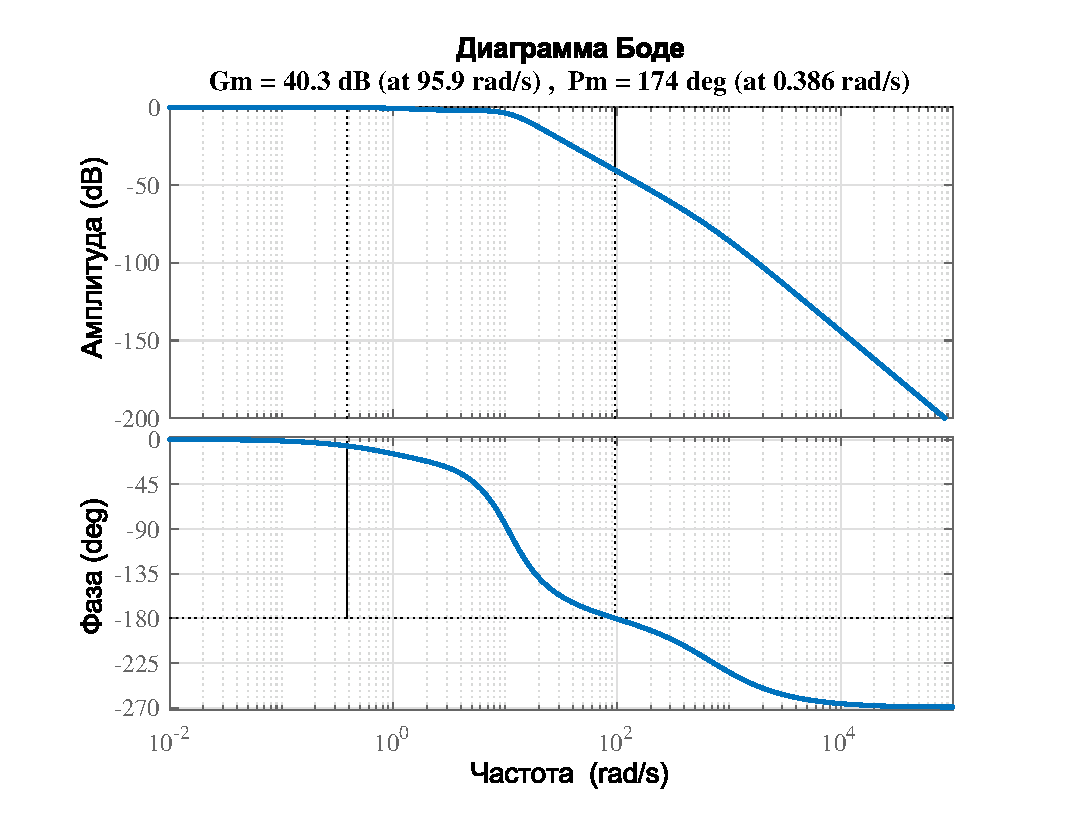
\includegraphics[scale = 0.4]{Bode.eps}}
    \caption{Диаграмма Боде}
\end{figure}
 
 Данные показатели удовлетворяют указанным условиям.\\
 
 Кроме того, удалось определить влияние возмущения $D(s)=Q/s$  на выходную переменную $Y(s)$. Для этого было необходимо было рассмотреть выходной сигнал при нулевом входном воздействии и ненулевом возмущении:
  \begin{figure}[h!]
    \center{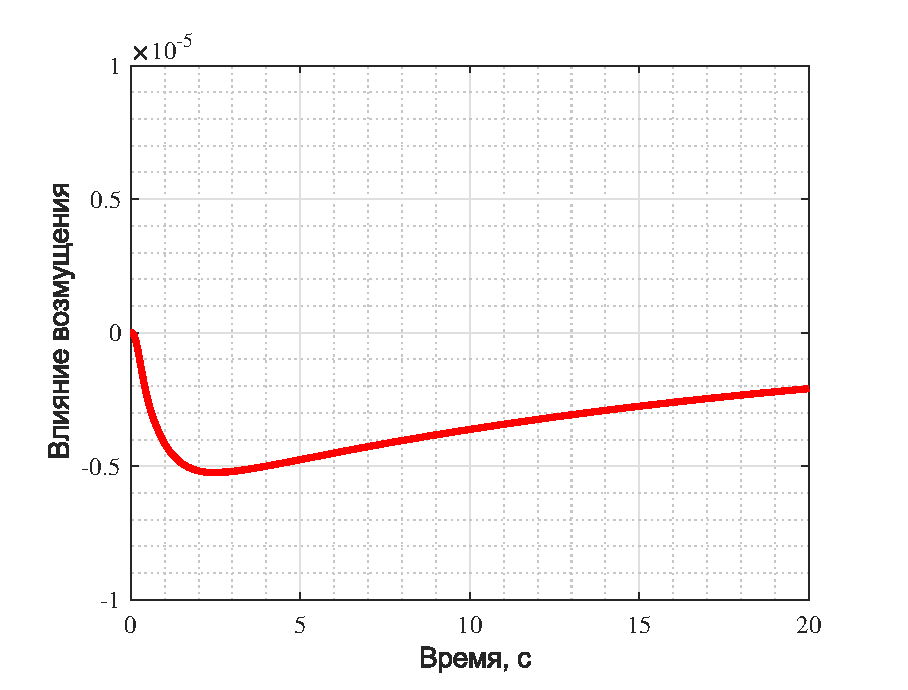
\includegraphics[scale = 0.7]{Dist.eps}}
    \caption{Влияние возмущения на выходной сигнал}
\end{figure}
 
\section{Дополнительное исследование системы}

Было исследовано поведение при входном ступенчатом сигнале с амплитудой 10, и тремя последовательными импульсами возмущения с амплитудами 10,10 и -10.
  \begin{figure}[h!]
    \center{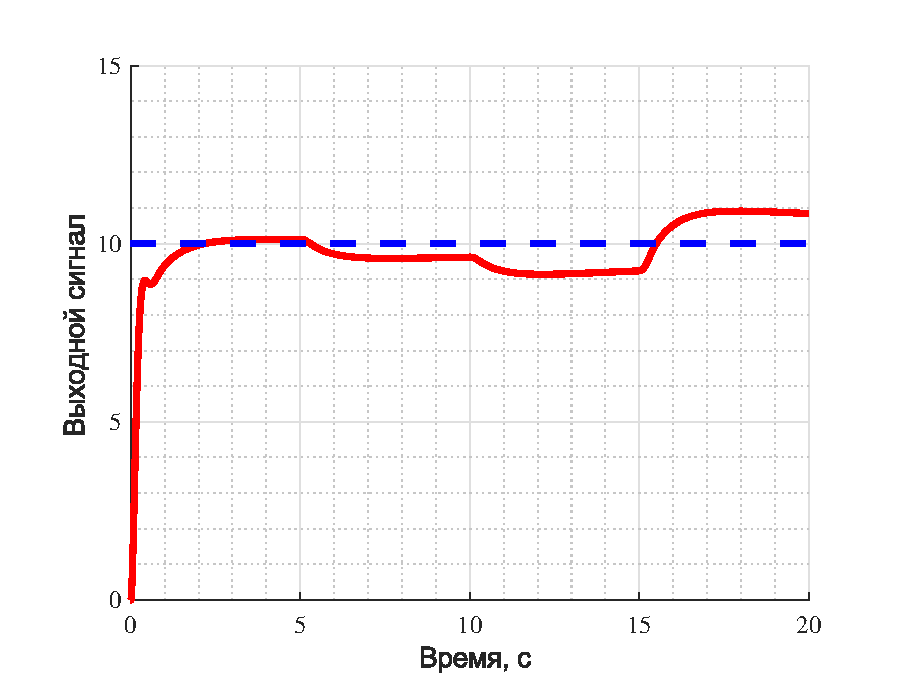
\includegraphics[scale = 0.7]{ManySteps.eps}}
    \caption{Влияние ступенчатого возмущения на выходной сигнал}
\end{figure}

\section{Вывод}
\begin{itemize}
\item Удалось синтезировать ПИД-регулятор, удовлетворяющий заданным условиям;
\item Дополнительное иссоелование системы позволяет говорить об устойчивости системы, достигнутой благодаря синтезу регулятора.
 \end{itemize}

\newpage
\section{Список используемой литературы} 
$[1]$ Дорф Р., Бишоп Р. Современные системы управления. М.: Лаборатория базовых знаний, Юнимедиастайл, 2002\\
$[2]$ Филлипс Ч., Харбор Р. Системы управления с обратной связью. – М.: Лаборатория базовых знаний, 2001. 616 с.\\
$[3]$ Control Tutorials for MATLAB and Simulink (CTMS) [Электронный ресурс] http://ctms.engin.umich.edu/CTMS/index.php

\end{document} 